\begin{center}
    

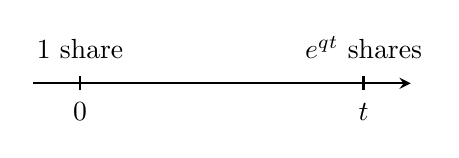
\begin{tikzpicture}[scale=0.6, thick] % <--- 在这里修改 scale 的数值来调整大小

    % --- 定义变量 ---
    % 定义 t 点在 x 轴上的位置，方便修改距离
    % 这里设置为 6cm，你可以根据需要调整这个数字
    \def\tpos{6}

    % --- 1. 绘制数轴主体 ---
    % draw 命令画线。
    % -> 表示末端有箭头。
    % >=stealth 设置箭头的样式为一种比较现代的风格。
    % 从坐标 (-1, 0) 画到 (\tpos + 1, 0)，两端稍微延伸一点比较美观。
    \draw[->, >=stealth] (-1, 0) -- (\tpos + 1, 0);


    % --- 2. 处理 "0" 点 ---
    % (a) 画刻度线 (Tick mark)
    % 在 x=0 处画一条短竖线，从 y=0.15 到 y=-0.15
    \draw (0, 0.15) -- (0, -0.15);

    % (b) 下方标 "0"
    % node 是一个放置文本或公式的节点。
    % [below] 表示位于指定坐标的下方。
    \node[below] at (0, -0.2) {$0$};

    % (c) 上方标 "1 share"
    % [above] 表示位于指定坐标上方。
    % y 坐标设置得比刻度线高一点 (0.3)，避免重叠。
    \node[above] at (0, 0.3) {1 share};


    % --- 3. 处理 "t" 点 ---
    % (a) 画刻度线
    % 在 x=\tpos 处画短竖线
    \draw (\tpos, 0.15) -- (\tpos, -0.15);

    % (b) 下方标 "t"
    \node[below] at (\tpos, -0.2) {$t$};

    % (c) 上方标 "e^{qt} shares"
    % 注意公式要放在两个 $ 符号之间
    \node[above] at (\tpos, 0.3) {$e^{qt}$ shares};

\end{tikzpicture}
\end{center}